\documentclass[12pt]{article}
\usepackage[utf8]{inputenc}
\usepackage{latexsym,amsfonts,amssymb,amsthm,amsmath}
\usepackage{float}
\usepackage{caption}
\usepackage{marginnote}
\usepackage{enumerate}
\usepackage{tikz}

\setlength{\parindent}{0in}
\setlength{\oddsidemargin}{0in}
\setlength{\textwidth}{6.5in}
\setlength{\textheight}{8.8in}
\setlength{\topmargin}{0in}
\setlength{\headheight}{18pt}

\newtheorem*{answer*}{Answer}
\newtheorem*{solution*}{Solution}
\newtheorem{remark}{Remark}

\renewcommand{\angle}{\measuredangle}

\title{Weekly Homework 7}
\author{Math Gecs}
\date{March 8, 2024}

\begin{document}
\maketitle

\subsection*{Exercise 1}
Consider two circles $S_1$ and $S_2$ centered at $A$ and $B$ and with radii $\sqrt{6}$ and $\sqrt{3} - 1$, respectively. Suppose that the two circles intersect at two distinct points $C$ and $D$. Suppose further that the two centers $A$ and $B$ are of distinct 2 apart. The sketch below is not to scale.


\begin{figure}[H]
        \centering
        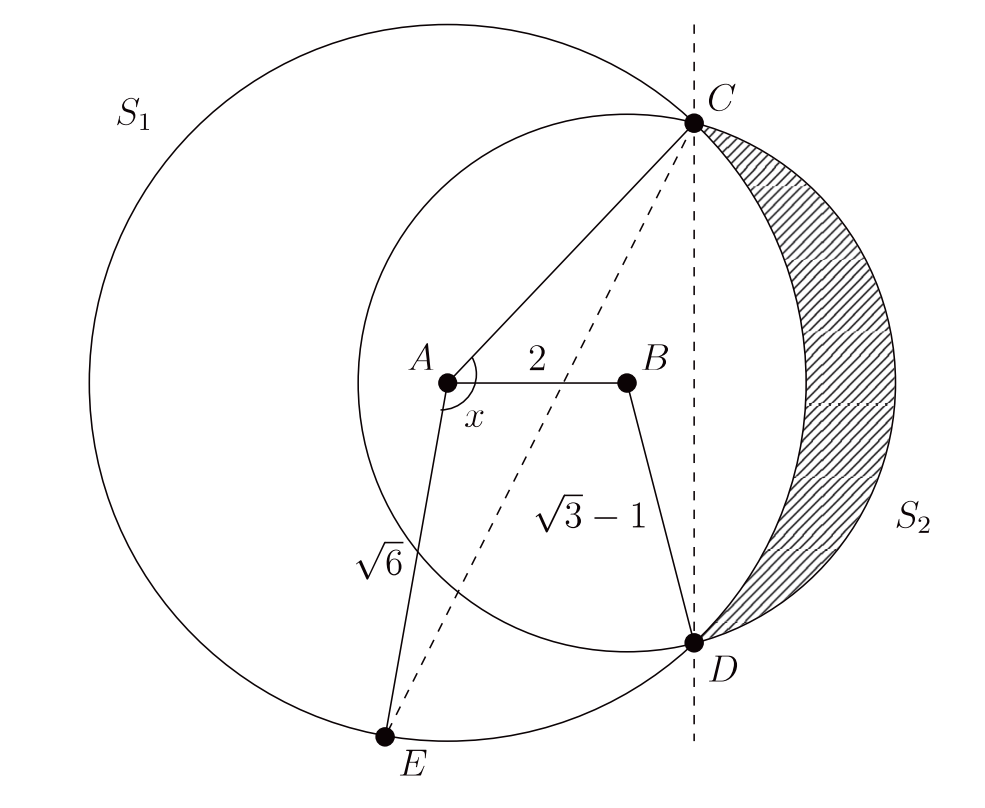
\includegraphics[width=12cm]{oxford_mat.png}
        \label{fig:oxford-MAT}
    \end{figure}

\begin{enumerate}[i]
    \item Find the angle $\angle CBA$, and deduce that $A$ and $B$ lie on the same side of the line $CD$.

    \item Show that $CD$ has length $3 - \sqrt{3}$ and hence calculate the angle $\measuredangle CAD$

    \item Show that the area of the region lying inside the circle $S_2$ and outside of the circle $S_1$ (that is the shaded region in the picture) is equal to.

    \item Suppose that a line through $C$ is drawn such that the total area covered by $S_1$ and $S_2$ is split into two equal areas. Let $E$ be the intersection of this line with $S_1$ and $x$ denote the angle $\angle CAE$. You may assume that $E$ lies on the larger arc $CD$ of $S_1$. Write down an equation which $x$ satisfies and explain why there is a unique solution $x$.
    
    \end{enumerate}

Source: Oxford MAT 2018 (Problem 4)\\

\begin{solution*}
(Type your solutions here.)
\end{solution*}

\vspace{2in}






\subsection*{Exercise 2}
How many integers between 100 and 999, inclusive, have the property
that some permutation of its digits is a multiple of 11 between 100
and 999 ? For example, both 121 and 211 have this property.

$\textbf{(A) } 226 \qquad \textbf{(B) } 243 \qquad \textbf{(C) } 270 \qquad \textbf{(D) } 469 \qquad \textbf{(E) } 486$
\\

Source: 2017 AMC 10A Problem 25\\

\begin{answer*}
$A$
\end{answer*}

\begin{solution*}
There are $81$ multiples of $11$ between $100$ and $999$ inclusive. Some have digits repeated twice, making $3$ permutations.
\\ \\
Others that have no repeated digits have $6$ permutations, but switching the hundreds and units digits also yield a multiple of $11$. Switching shows we have overcounted by a factor of $2$, so assign  $6 \div 2 = 3$ permutations to each multiple.
\\ \\
There are now $81*3 = 243$ permutations, but we have overcounted*. Some multiples of 11 have $0$ as a digit. Since $0$ cannot be the digit of the hundreds place, we must subtract a permutation for each. 
\\ \\
There are $110, 220, 330 ... 990$, yielding $9$ extra permutations
\\ \\
Also, there are $209, 308, 407...902$, yielding $8$ more permutations.
\\ \\
Now, just subtract these $17$ from the total $(243)$ to get $226$. $\boxed{\textbf{(A) } 226}$
\\ \\
*If short on time, observe that $226$ is the only answer choice less than $243$, and therefore is the only feasible answer.
\end{solution*}


\begin{solution*}
    We note that we only have to consider multiples of $11$ and see how many valid permutations each has. We can do casework on the number of repeating digits that the multiple of $11$ has:
\\ \\
$\textbf{Case 1:}$ All three digits are the same. 
By inspection, we find that there are no multiples of $11$ here.
\\ \\
$\textbf{Case 2:}$ Two of the digits are the same, and the third is different.
\\ \\
$\textbf{Case 2a:}$
There are $8$ multiples of $11$ without a zero that have this property:
$121$, $242$, $363$, $484$, $616$, $737$, $858$, $979$.
Each contributes $3$ valid permutations, so there are $8 \cdot 3 = 24$ permutations in this subcase.
\\ \\
$\textbf{Case 2b:}$
There are $9$ multiples of $11$ with a zero that have this property:
$110$, $220$, $330$, $440$, $550$, $660$, $770$, $880$, $990$.
Each one contributes $2$ valid permutations (the first digit can't be zero), so there are $9 \cdot 2 = 18$ permutations in this subcase.
\\ \\
$\textbf{Case 3:}$ All the digits are different.
Since there are $\frac{990-110}{11}+1 = 81$ multiples of $11$ between $100$ and $999$, there are $81-8-9 = 64$ multiples of $11$ remaining in this case. However, $8$ of them contain a zero, namely $209$, $308$, $407$, $506$, $605$, $704$, $803$, and $902$. Each of those multiples of $11$ contributes $2 \cdot 2=4$ valid permutations, but we overcounted by a factor of $2$; every permutation of $209$, for example, is also a permutation of $902$. Therefore, there are $8 \cdot 4 / 2 = 16$. Therefore, there are $64-8=56$ remaining multiples of $11$ without a $0$ in this case. Each one contributes $3! = 6$ valid permutations, but once again, we overcounted by a factor of $2$ (note that if a number ABC is a multiple of $11$, then so is CBA). Therefore, there are $56 \cdot 6 / 2 = 168$ valid permutations in this subcase.
\\ \\
Adding up all the permutations from all the cases, we have $24+18+16+168 = \boxed{\textbf{(A) } 226}$.
\\ 
\end{solution*}

\begin{solution*}
    We can first overcount and then subtract.
We know that there are $81$ multiples of $11$.
\\ \\
We can then multiply by $6$ for each permutation of these multiples. (Yet some multiples do not have six distinct permutations.)
\\ \\
Now divide by $2$, because if a number $abc$ with digits $a$, $b$, and $c$ is a multiple of $11$, then $cba$ is also a multiple of $11$ so we have counted the same permutations twice. 
\\ \\
Basically, each multiple of $11$ has its own $3$ permutations (say $abc$ has $abc$ $acb$ and $bac$ whereas $cba$ has $cba$ $cab$ and $bca$). We know that each multiple of $11$ has at least $3$ permutations because it cannot have $3$ repeating digits.
\\ \\
Hence we have $243$ permutations without subtracting for overcounting.
Now note that we overcounted cases in which we have $0$'s at the start of each number. So, in theory, we could just answer $A$ and then move on.
\\ \\
If we want to solve it, then we continue.
\\ \\
We overcounted cases where the middle digit of the number is $0$ and the last digit is $0$.
\\ \\
Note that we assigned each multiple of $11$ three permutations.
\\ \\
The last digit is $0$ gives $9$ possibilities where we overcounted by $1$ permutation for each of $110, 220, ... , 990$.
\\ \\
The middle digit is $0$ gives $8$ possibilities where we overcount by $1$.
$605, 704, 803, 902$ and $506, 407, 308, 209$
\\ \\
Subtracting $17$ gives $\boxed{\textbf{(A) } 226}$.
\\ \\
Now, we may ask if there is further overlap (i.e if two of $abc$ and $bac$ and $acb$ were multiples of $11$). Thankfully, using divisibility rules, this can never happen, as taking the divisibility rule mod $11$ and adding, we get that $2a$, $2b$, or $2c$  is congruent to $0\ (mod\ 11)$. Since $a, b, c$ are digits, this can never happen as none of them can equal $11$ and they can't equal $0$ as they are the leading digit of a three-digit number in each of the cases.
\\ \\
\end{solution*}

\end{document}